\documentclass{beamer}
\usetheme{Berkeley}

% this allows code highlighting
\usepackage{listings}

% set noident for whole file
%\setlength\parindent{0pt}

% vertical aligned tabular
\usepackage{tabularx}
\def\tabularxcolumn#1{m{#1}}

% http://www.latex-community.org/forum/viewtopic.php?f=5&t=6581
% this helps set the outline names (versus numbers)
\newcommand{\sectiontitle}{}
\newcommand{\newsection}[1]{\renewcommand{\sectiontitle}{#1}\section{#1}}
\newcommand{\subsectiontitle}{}
\newcommand{\newsubsection}[1]{\renewcommand{\subsectiontitle}{#1}\subsection{#1}}

% change beamer sizes
\def\miniscule{\fontsize{4pt}{5pt}\selectfont}
\def\miniminiscule{\fontsize{4pt}{5pt}\selectfont}
\setbeamerfont{author in sidebar}{size=\tiny}
\setbeamerfont{section in sidebar}{size=\miniscule}
\setbeamerfont{subsection in sidebar}{size=\def\miniminiscule}
\setbeamerfont{title in sidebar}{size=\tiny}

% http://tex.stackexchange.com/questions/26712/how-to-make-outline-frame-in-beamer
% http://tex.stackexchange.com/questions/28654/beamer-table-of-contents-display-all-subsections-below-section
% generate table of contents ("outlines") for each new section
%\AtBeginSection[]
%{
%  \begin{frame}<beamer>
%    \frametitle{\sectiontitle}
%    \tableofcontents[currentsection]
%  \end{frame}
%}

\AtBeginSubsection[]
{
  \begin{frame}<beamer>
    \frametitle{\subsectiontitle}
    \tableofcontents[currentsection,currentsubsection]
  \end{frame}
}

% title page info
\title{PCR Primer Validation Report}
\subtitle{Exploring the potential for false negatives in PCR design}
\author{Aaron C. Robinson}
\date{\today} % so that it is updated on generation

\begin{document}

  % generates titlepage
  \maketitle

  \newsection{Send Blast}
  \begin{frame}
    \frametitle{Send Blast}
    \framesubtitle{Blast bait sequences against NCBI}
    
    \begin{tabularx}{\textwidth}{l X}
    	  \hspace{-.35cm} Utilizes in-house tool suite called blast2tree. & 
\includegraphics[scale=.25]{ncbi_blast}
    \end{tabularx} \\ \hfill \\

    Filtering \& Bounding:
    
	\begin{itemize} \itemsep1em
	  \item 1500 hits are collected
	  \item Sequences longer than 1000 nucleotides are downloaded from GenBank
	  \item Only results from our target organism are considered
	\end{itemize}
	
  \end{frame}
  
  \newsection{Trim Database}
  \begin{frame}
    \frametitle{Trim Database}
    \framesubtitle{Filter and build Fastas from Blast results}
    
	By this point,
	
	\begin{enumerate} \itemsep1em
	  \item Blast results have been converted to csv
	  \item The csv results have been imported into SQLite database
	\end{enumerate}
	
	\vspace{-1cm} \begin{center}
	  \line(1,0){300}
	\end{center}
	
	Given a database containing Blast results, this script builds FASTA files for pair-wise alignment:
    
    \begin{itemize} \itemsep1em
	  \item A filter of 1e-9 (or $10^(-10)$) is used to screen results
	  \item Sequences that pass the filter are converted to FASTA
	\end{itemize}
	
    %More content goes here
  \end{frame}
  
  \newsection{Pairwise Alignment}
  \begin{frame}
    \frametitle{Pairwise Alignment}
    \framesubtitle{Forward and reverse primers are pairwise-aligned using SSearch36}
    
	At this point, we need to perform a pairwise alignment to determine the primer region of our result sequences.    
    
    \begin{itemize} \itemsep1em
    	  \item A pairwise alignment is performed against the screened Blast results and each primer
    	  \item SSearch36 is part of the Fasta36 alignment tools, using a Smith-Waterman algorithm
    \end{itemize}

	This returns a format that is parsed into CSV and imported into SQLite3.
    
  \end{frame}
  
  \newsection{Generate Report}
  \newsubsection{Outline}
  \begin{frame}
    \frametitle{Generate Report}
    \framesubtitle{Using Python and Jinja2, the results are parsed into HTML report}
    
	This process...
	
	\begin{itemize} \itemsep.5em
	  \item encompasses the majority of the report generation
	  \item is standalone given the SQLite databases are built  
	\end{itemize}
	
	By now the SQLite database should contain three tables:
	
	\begin{itemize} \itemsep.5em
	  \item blast\_results
	  \item 'ssearch\_forward'
	  \item 'ssearch\_reverse'
	\end{itemize}    
    
  \end{frame}
  
  \begin{frame}
    \frametitle{Generate Report}
    \framesubtitle{Using Python and Jinja2, the results are parsed into HTML report}
    
	We will count 100\% matches but they will not be iterated for reporting purposes. \\ \hfill \\ 
	
	Therefore for the result of the process refer only to mismatches. \\ \hfill \\ 
    
	Filtering:
	
	\begin{itemize} \itemsep.5em
	  \item A filter of 1e-4 (or $10^(-5)$) is used to screen results
	  \item We verify the alignment is over the full primer region
	\end{itemize}
    
  \end{frame}
  
  \newsubsection{Report HTML}
  \begin{frame}
    \frametitle{Report HTML}
    \framesubtitle{This is the HTML output from the Primer Report}
    \begin{figure}[htp]
	\centering
	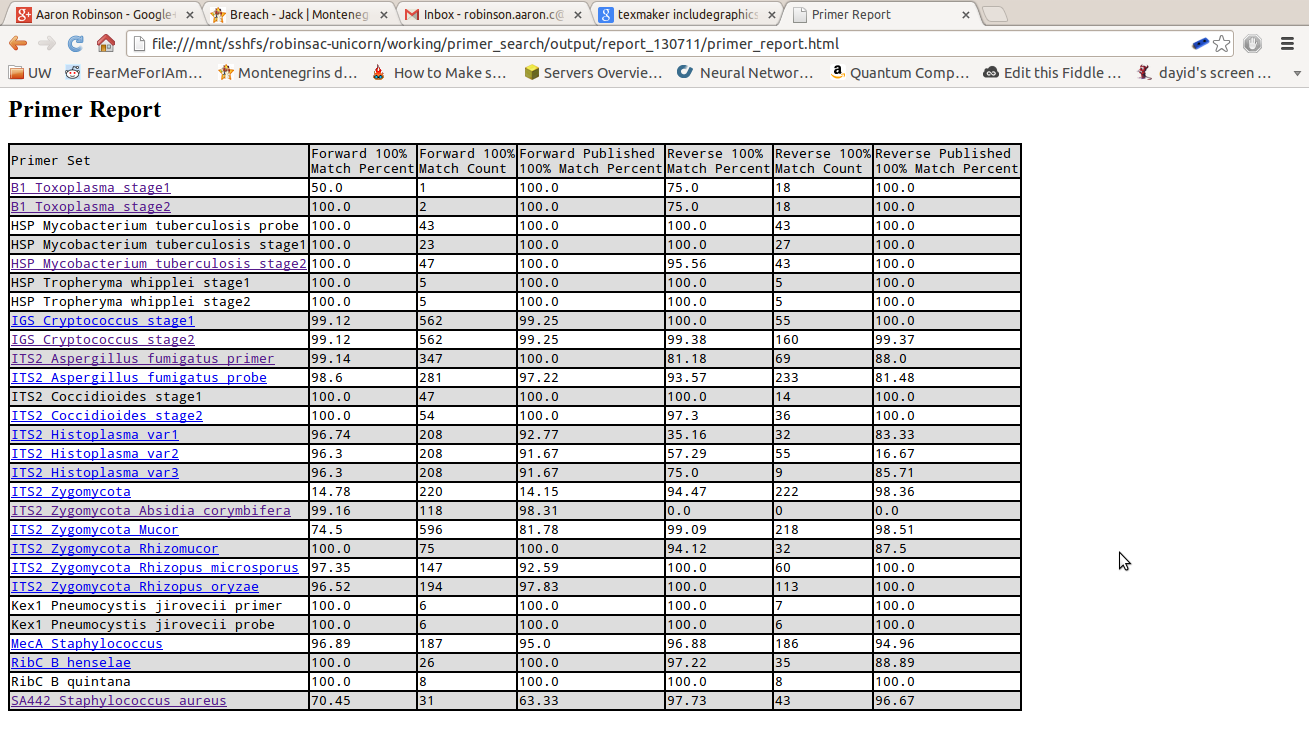
\includegraphics[width=1\textwidth]{primer_report}
	\caption{This is an example of 'primer\_report.html'}\label{fig:primer_report}
	\end{figure}
  \end{frame}
  
  \newsubsection{Organism HTML}
  \begin{frame}
    \frametitle{Organism HTML}
    \framesubtitle{This is the organism specific report}
    \begin{figure}[htp]
	\centering
	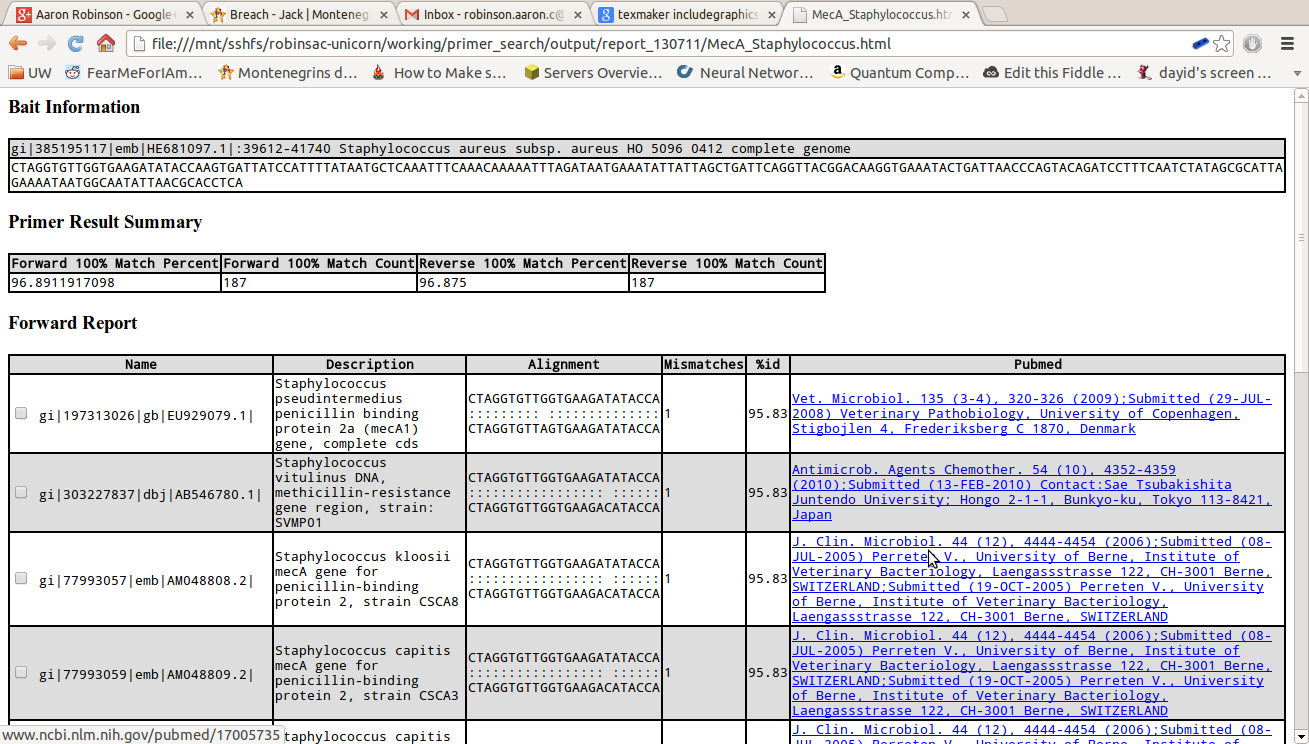
\includegraphics[width=1\textwidth]{meca_details}
	\caption{This is an example output for the MecA gene given S. aurous }\label{fig:meca_details}
	\end{figure}
  \end{frame}
  
  \newsection{BASH it}
  \begin{frame}
    \frametitle{BASH it}
    \framesubtitle{Pipe it all together using a BASH script}
    
    \begin{itemize} \itemsep1em
      \item There are many scripting options for connecting all the peices.
      \item A BASH script was used for it's ability to facilitate a fast path to solution.
      \item Moving forward, a Python wrapper would be a more elegant solution.
    \end{itemize}
    
  \end{frame}
  
  \newsection{Questions}
  \begin{frame} 
    \frametitle{Questions}
    \framesubtitle{Please feel free to critique how this process could be improved}
    
    
\includegraphics[width=1\textwidth]{ask-question}
  \end{frame}

\end{document}